\section{Learning Methods}\label{sec:allocation}

\subsection{Q-Learning for Capital Allocation}\label{sec:14}

The outer learner combines the funded strategy portfolios under fixed or learned entry sizing. Section~\ref{sec:11} explains the shared entry-sizing procedure. It makes a different decision: what fraction of one \$10 million budget should track each funded strategy? Its seven put/straddle targets are 100/0, 90/10, 75/25, 50/50, 25/75, 10/90 and 0/100. Weights sum to one; there is no outer leverage or cash action. A weekly decision based on prior-close information takes effect at the next close. The first session retains old holdings, then positions resize and drift until the next decision.


\subsubsection*{State and Action Spaces}

Nine state inputs describe four economic opportunities---put-spread rank strength, the put implied-versus-realized variance gap, straddle IV-versus-RV richness and completed straddle premium---plus relative strategy volatility, strategy-return correlation, VIX, relative recent Sharpe and previous straddle weight. Previous holdings matter because changing allocations incurs additional costs. A target is a fractional claim on a funded strategy index, not a new integer-contract order book. Underlying trading costs remain embedded in source returns; resizing adds source-based option and hedge charges.


\begin{equation*}R_w(\lambda)=\sum_{d\in w}(z_d-\lambda z_d^2),\qquad z_d=e_d/\widehat{\sigma}_{\mathrm{ref}}\end{equation*}

\subsubsection*{Reward Specification and Fitted Q Iteration}

Reference volatility is estimated from the training window's fixed-50/50 excess returns. The parameter \(\lambda\) penalizes squared normalized fluctuations. At \(\lambda\) = 0, the directive is profit alone: additional normalized return earns reward without an explicit charge for the accompanying volatility. A higher-profit, higher-variance strategy can therefore attract capital even when its risk-adjusted performance is weaker. This objective does not maximize Sharpe. The discount \(\gamma\) = 0.99 separately weights continuation value; it is unchanged across risk preferences.


Monthly fitted Q iteration uses the preceding 104 completed weeks, with at least 52. A quadratic function of straddle weight has coefficients linear in standardized state, giving 30 coefficients. Each Bellman update regresses immediate reward plus discounted next-state maximum value onto the same basis \cite{ernst2005}. We use ridge coefficient 10 and 200 updates. Seven prior allocations crossed with seven actions supply counterfactual paths on each market week; they do not create independent market observations.


Q uses 50/50 before enough training weeks exist; each fixed control starts at its own target. A discount-zero learner supplies a matched one-period control. In the factorial experiment, Q is refitted independently for each entry policy. Strategy-dependent risk features, reward paths and resizing charges are rebuilt for that policy, while economic signal definitions remain shared.


The outer experiment holds each signal's proposals fixed while learning how to combine their exposures. Entry sizes change the inner funded portfolios; Q changes the capital assigned across them. The accounting layers are deliberately distinct, allowing us to remove either learning layer in the four-way comparison.


\FloatBarrier
\subsection{Contextual Bandit Entry Sizing}\label{sec:11}

We use direct policy search to learn a contextual sizing policy that maximizes historical portfolio Sharpe. The rule fixes direction and contracts; the bandit chooses 50\%, 75\% or 100\% exposure. CEM optimizes the put policy.


\subsubsection*{Regression Tree and Cross-Entropy Policy Search}

Each monthly regression tree uses completed examples from the preceding 18 months. Its target is cumulative full-size profit above cash; splits reduce prediction error across 27 inputs. At most eight leaves define states. With n examples, minimum leaf count is max(8, min(63, floor(n/8))); fewer than 16 use full size.


\begin{figure}[!htbp]\centering
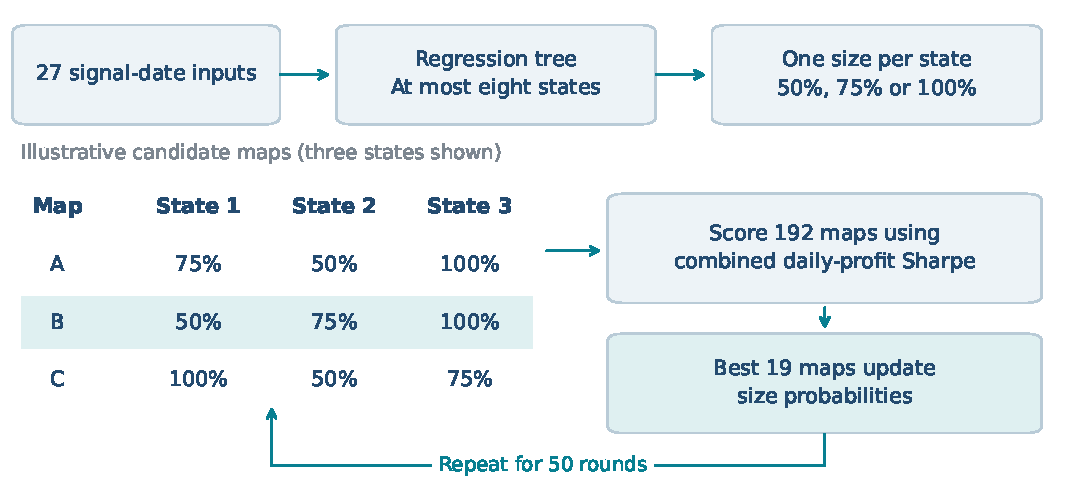
\includegraphics[width=\linewidth]{entry_policy.pdf}
\caption{The original tree/CEM construction. The three-state maps illustrate candidates; actual trees have up to eight states. Each candidate selects action-specific completed paths; the best 19 update sampling probabilities. The retained map sizes next month's proposals.}\label{fig:entry-policy}
\end{figure}

For completed example i, p denotes its profit above cash on day d at size a. Each size has its own rounded contracts and simulated hedge path. A map assigns one size to each tree state. We sum its daily paths, retaining overlapping positions and zero-profit sessions, and score the result:


\begin{equation*}g_d(m)=\sum_i p_{i,d}(a_{\ell(x_i)}),\qquad\widehat S_{\rm train}(m)=\sqrt{252}\,\overline{g}/s_g.\end{equation*}

CEM \cite{deboer2005} updates size probabilities toward the best 19 of 192 candidate maps for 50 rounds. Constant maps and the incumbent are anchors. This standalone-path training score differs from funded-account Sharpe: replay additionally applies shared cash, inventory and admission.


The 27-input, 18-month specification was retained from 33 archived configurations ranked on 2018--2021 validation scores. Archived selection used a \$345 million research account; the funded comparisons below use \$10 million. Detailed feature experiments and the refitting timeline are in Appendix~\ref{app:g}; exact fitting settings are in Appendix~\ref{app:b}.

\subsubsection*{Ridge Regression and Context-Based Sizing}

The straddle bandit fits a 60-month ridge model to completed full-size profit, using 14 inputs and requiring 128 examples. The inputs include IV, RV-IV memory, VIX and a separate fixed-half paper portfolio's recent performance. Score terciles define three states. We enumerate all 27 size maps and retain the highest training Sharpe. Insufficient history uses half size. Both learners use completed outcomes; Appendix~\ref{app:b} provides exact fitting details.




The policy chooses 50\%, 75\% or 100\% exposure within the same completed-path Sharpe framework used for put pairs. The ridge score groups opportunities; the selected context-to-size map determines the requested size and need not increase monotonically with the score. The model uses completed quote-available labels: 4,116 training rewards are finite, while the policy handles all 35,774 proposals. Section~\ref{sec:13} reports feature-usage and admission diagnostics.
\FloatBarrier
